\documentclass[a4paper,12pt]{article}
\usepackage[utf8]{inputenc}
\usepackage[slovene]{babel}
\usepackage{amsmath}
\usepackage{graphicx}
\usepackage{booktabs}
\usepackage{float}
\usepackage{biblatex} %Imports biblatex package
\usepackage[backend=biber,style=numeric]{biblatex} % or any style you prefer
\addbibresource{predstavitev.bib}

% Komanda za vrednost z aboslutno napako
\newcommand{\abserr}[5]{
    \ensuremath{#1_{#2} = (#3 \ \pm \ #4) \ #5}
}

\newcommand{\relerr}[5]{
    \ensuremath{#1_{#2} = #3 \ (1 \pm \ #4) \ #5}
}

\newcommand{\relativna}[3]{
    \ensuremath{#1 \ (1 \pm #2) \ #3}
}

\newcommand{\absolutna}[3]{
    \ensuremath{(#1 \ \pm \ #2) \ #3}
}


\title{Optična rotacija raztopine saharoze}
\author{Matija Zanjkovič, Mesarec Tilen, Petauer Maja}
\date{Junij 2025}

\begin{document}
\maketitle

\section*{Uvod}

Pri naši projektni nalogi smo raziskovali optično rotacijo polarizirane svetlobe. \\\\

Kaj pa sploh je optična rotacija in zakaj se pojavi?

Dve molekuli, ki sta zrcalni sliki drugi drugi in se ne moreta prekrivati, imenujemo enantiomerni par.
\begin{center}
    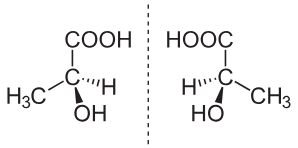
\includegraphics[width=0.5\textwidth]{slike/enantiomer.png}
\end{center}

Po tej definiciji voda tako ni enantiomer, ker je smimetrična in se njena slika prekriva z njo.
\begin{center}
    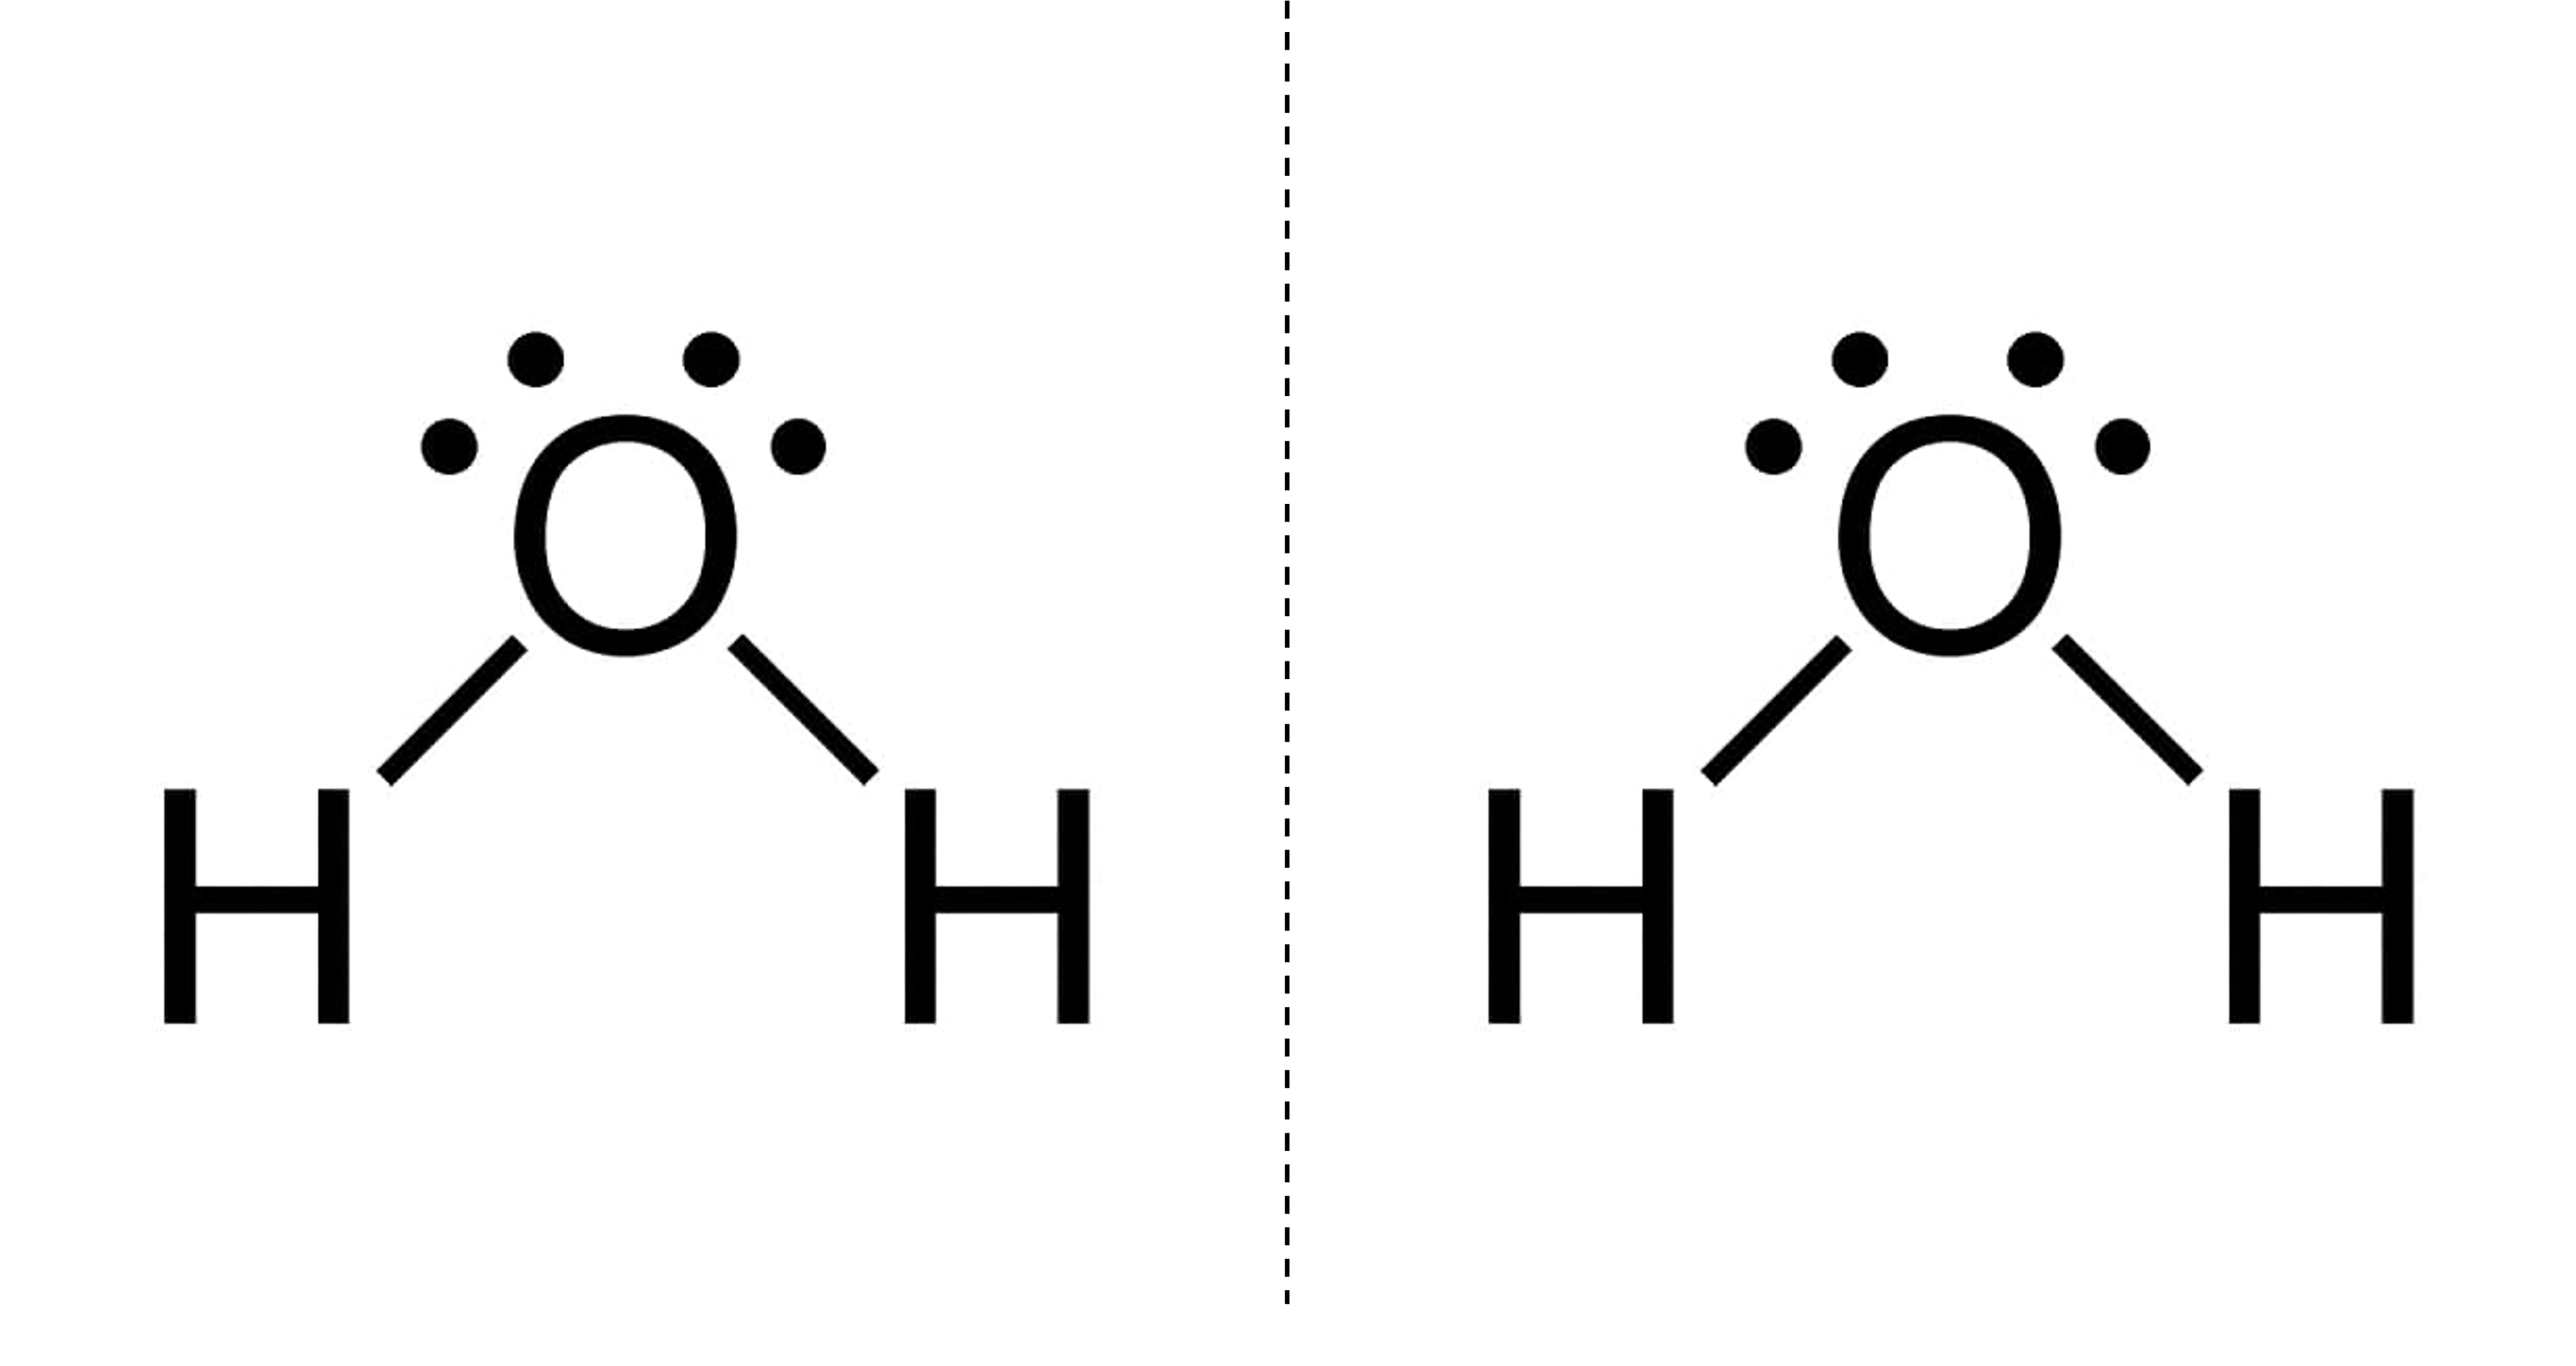
\includegraphics[width=0.5\textwidth]{slike/voda.png}
\end{center}

Molekule slakdkorjev, ko so glukoza, fruktoza in saharoza pa so izomeri, kar pomeni, da imajo enantiomere. Latnost enantiomernih molekul 
se imenuje kiralnost.
Ločeni enantiomeri imajo enake lastnosti v akiralenem okolju - to pomeni, da imajo enako topnost, fizikalne in spektroskopske lastnosti ter enako kemijsko reaktivnost z akiralnimi reagenti.

Vendar pa imajo v kiralnem okolju različne lastnosti. Enantiomeri reagirajo z različno hitrostjo z kiralnimi reagenti in se različno odzivajo na kiralne katalizatorje. Pogosto povzročajo tudi različne fiziološke učinke, saj so biološki receptorji kiralni.
Na primer, vonj R-enantiomera karvona (olja zelene mete) in S-enantiomera (olja kumine) je zelo različen. Fizikalna lastnost kiralnih molekul, ki pa je zanimala nas pa je optična rotacija.
Enantiomeri spolarizirano svetlobo rotirajo z isto mero a v nasprotni smeri. Če so ti enantiomeri v enakih koncentracijah, se njihova optična rotacija izniči.

Ker pa molekule glukoze, fruktue in saharoze v naravi nimajo prisotnega enantiomera, pomeni da so optično aktivne in lahko rotirajo polarizirano svetlobo. Prav to smo raziskovali v naši projektni nalogi.

\section*{Teorija}

Specifično rotacijo $\alpha$ definiramo kot količnik med kotom rotacije $\alpha$ in produktom koncentracije $c$ in dolžine cevi $l$:
\[
[\alpha]^{\text{T}}_{\lambda}= \frac{\alpha}{c \cdot l}
\]

Pri tem smo merili v enotah $\alpha$ v stopinjah, $c$ v g/mL in $l$ v dm, torej je enota specifične rotacije 
\[
\left[ [\alpha] \right] = \left[ \frac{^\circ \cdot \mathrm{dm}}{\mathrm{g} \cdot \mathrm{mL}} \right]
\]


Naš prvi cilj je bil izmeriti specifično rotacijo saharoze v vodi pri različnih koncentracijah in dveh valovnih dolžinah (rdeča in zelena).
Kot drugi cilj pa smo želeli preveriti Drudejev model disperzije, ki opisuje odvisnost specifične rotacije od valovne dolžine svetlobe.

\section*{Izvedba eksperimenta}

Raztopino saharoze smo pripravili s tehtanjem potrebne količine sladkorja, ki smo ga nato raztopili v vodi. Za vsako koncentracijo smo pripravili 3000 mL raztopine, ki smo jo nato vlili v 11.5 cm dolgo pleksi cev.
Pleksi cev je bila na vsaki strani zaprata s akrilnim steklom. Na eni strani smo imeli linearni polarizator, ki je bil fiksen in na drugi strani pa smo imeli rotirajoči polarizator, ki smo ga lahko obračali in tako merili kot rotacije svetlobe.
Z laserjem smo nato posvetili skozi cev in merili kot rotacije svetlobe pri različnih koncentracijah saharoze in dveh valovnih dolžinah (rdeča in zelena). Rotacijo smo določili s 
pomočjo metrilnika specifične intenzitete svetlobe, ki je bil povezan z računalnikom na LoggerPro programu. Kot rotacije smo določili tako, da smo poiskali maksimum intenzitete svetlobe 


\section*{Merjene količine}
\begin{itemize}
    \item Koncentracija saharoze $c$ (g/mL)
    \item Valovna dolžina $\lambda$ (nm)
    \item Kot rotacije $\alpha$ (°)
    \item Dolžina cevi $l$ (dm)
\end{itemize}


Dolžina cevi:
\[
\abserr{L}{}{11.5}{0.5}{\text{dm}}
\]
\[
\relerr{L}{}{11.5}{0.043}{\text{dm}}
\]

% Volumen raztopine
Volumen raztopine je bil:
\[
\abserr{V}{}{3000}{60}{\text{mL}}
\]
\[
\relerr{V}{}{3000}{0.02}{\text{mL}}
\]

To smo počeli pri konstantni temperaturi $T = 22 \pm 1 \, \text{°C}$, saj 
na specifično rotacijo vpliva tudi temperatura.\\\\

% Masa saharoze
Masa saharoze je bila izmerjena z napako $3\,\text{g}$. Relativna napaka koncentracije:

\begin{table}[H]
\centering
\begin{tabular}{ccc}
\toprule
$c$ [g/mL] & $\sigma c$ \\
\midrule
0.000 & -- \\
0.030 & 0.033 \\
0.050 & 0.020 \\
0.070 & 0.014 \\
0.090 & 0.011 \\
0.100 & 0.010 \\
\bottomrule
\end{tabular}
\caption{Relativna napaka koncentracije raztopine saharoze.}
\end{table}

Pri meritvah smo opazili, da je pleksi steklo na obeh straneh cevi povzročilo dodatno rotacijo svetlobe. Ta učinek smo upoštevali pri izračunu kotov rotacije.
\begin{table}[H]
\centering
\begin{tabular}{cccc}
\toprule
$c$ [g/mL] & $\alpha_r$ [°] & $\alpha_z$ [°] & $\Delta\alpha$ [°] \\
\midrule
0.000 & 75  & 79  & 2 \\
0.030 & 90  & 96  & 2 \\
0.050 & 102 & 110 & 2 \\
0.070 & 115 & 126 & 2 \\
0.090 & 131 & 136 & 2 \\
0.100 & 137 & 141 & 2 \\
\bottomrule
\end{tabular}
\caption{Izmerjeni koti rotacije za rdečo ($\alpha_r$) in zeleno ($\alpha_z$) svetlobo.}
\end{table}

Meritve z odšteto začetno vrednostjo:

\begin{table}[H]
\centering
\begin{tabular}{cccccc}
\toprule
$c$ [g/mL] & $\alpha_r$ [°] & $\alpha_z$ [°]  & $\Delta \alpha$ [°] & $\sigma \alpha_r$ & $\sigma \alpha_z$ \\
\midrule
0.000 & 0  & 0 & 4 &  \\
0.030 & 15 & 17 & 4 & 0,26 & 0,24 \\
0.050 & 27 & 31 & 4 & 0,15 & 0,13 \\
0.070 & 40 & 47 & 4 & 0,10 & 0,09 \\
0.090 & 56 & 57 & 4 & 0,07 & 0,07 \\
0.100 & 62 & 64 & 4 & 0,06 & 0,06 \\
\bottomrule
\end{tabular}
\caption{Koti rotacije z odšteto začetno vrednostjo za rdečo ($\alpha_r$) in zeleno ($\alpha_z$) svetlobo.}
\end{table}


\section*{Izračun specifične rotacije}
\[
[\alpha] = \frac{\alpha}{c \cdot L}
\]
\begin{minipage}{0.48\textwidth}
\textbf{Rdeča:}
\begin{align*}
[\alpha]_{c=0.030} &= 43 \ (1 \pm 0.36) \ \frac{^\circ \cdot \mathrm{dm}}{\mathrm{g} \cdot \mathrm{mL}}\\
[\alpha]_{c=0.050} &= 47 \ (1 \pm 0.23) \ \frac{^\circ \cdot \mathrm{dm}}{\mathrm{g} \cdot \mathrm{mL}}\\
[\alpha]_{c=0.070} &= 50 \ (1 \pm 0.17) \ \frac{^\circ \cdot \mathrm{dm}}{\mathrm{g} \cdot \mathrm{mL}}\\
[\alpha]_{c=0.090} &= 54 \ (1 \pm 0.15) \ \frac{^\circ \cdot \mathrm{dm}}{\mathrm{g} \cdot \mathrm{mL}}\\
[\alpha]_{c=0.100} &= 54 \ (1 \pm 0.14) \ \frac{^\circ \cdot \mathrm{dm}}{\mathrm{g} \cdot \mathrm{mL}}\\
\end{align*}
\end{minipage}
\hfill
\begin{minipage}{0.48\textwidth}

\begin{align*}
[\alpha]_{c=0.030} &= (43 \pm 15) \ \frac{^\circ \cdot \mathrm{dm}}{\mathrm{g} \cdot \mathrm{mL}} \\
[\alpha]_{c=0.050} &= (47 \pm 11) \ \frac{^\circ \cdot \mathrm{dm}}{\mathrm{g} \cdot \mathrm{mL}} \\
[\alpha]_{c=0.070} &= (50 \pm 9)  \ \frac{^\circ \cdot \mathrm{dm}}{\mathrm{g} \cdot \mathrm{mL}}\\
[\alpha]_{c=0.090} &= (54 \pm 8)  \ \frac{^\circ \cdot \mathrm{dm}}{\mathrm{g} \cdot \mathrm{mL}}\\
[\alpha]_{c=0.100} &= (54 \pm 8)  \ \frac{^\circ \cdot \mathrm{dm}}{\mathrm{g} \cdot \mathrm{mL}}\\
\end{align*}
\end{minipage}

\vspace{1em}

\begin{minipage}{0.48\textwidth}
\textbf{Zelena:}
\begin{align*}
[\alpha]_{c=0.030} &= 49 \ (1 \pm 0.33) \ \frac{^\circ \cdot \mathrm{dm}}{\mathrm{g} \cdot \mathrm{mL}} \\
[\alpha]_{c=0.050} &= 54 \ (1 \pm 0.21) \ \frac{^\circ \cdot \mathrm{dm}}{\mathrm{g} \cdot \mathrm{mL}} \\
[\alpha]_{c=0.070} &= 58 \ (1 \pm 0.16) \ \frac{^\circ \cdot \mathrm{dm}}{\mathrm{g} \cdot \mathrm{mL}} \\
[\alpha]_{c=0.090} &= 55 \ (1 \pm 0.14) \ \frac{^\circ \cdot \mathrm{dm}}{\mathrm{g} \cdot \mathrm{mL}} \\
[\alpha]_{c=0.100} &= 56 \ (1 \pm 0.14) \ \frac{^\circ \cdot \mathrm{dm}}{\mathrm{g} \cdot \mathrm{mL}} \\
\end{align*}
\end{minipage}
\hfill
\begin{minipage}{0.48\textwidth}

\begin{align*}
[\alpha]_{c=0.030} &= (49 \pm 16) \  \frac{^\circ \cdot \mathrm{dm}}{\mathrm{g} \cdot \mathrm{mL}} \\
[\alpha]_{c=0.050} &= (54 \pm 11) \  \frac{^\circ \cdot \mathrm{dm}}{\mathrm{g} \cdot \mathrm{mL}} \\
[\alpha]_{c=0.070} &= (58 \pm 9)  \ \frac{^\circ \cdot \mathrm{dm}}{\mathrm{g} \cdot \mathrm{mL}} \\
[\alpha]_{c=0.090} &= (55 \pm 8)  \ \frac{^\circ \cdot \mathrm{dm}}{\mathrm{g} \cdot \mathrm{mL}} \\
[\alpha]_{c=0.100} &= (56 \pm 8)  \ \frac{^\circ \cdot \mathrm{dm}}{\mathrm{g} \cdot \mathrm{mL}} \\
\end{align*}
\end{minipage}


\section*{Povprečna specifična rotacija}

Za rdečo svetlobo:
\[
\overline{[\alpha]}_{\text{rdeča}} = \frac{43 + 47 + 50 + 54 + 54}{5} = 49.6 \approx 50
\]
Za zeleno svetlobo:
\[
\overline{[\alpha]}_{\text{zelena}} = \frac{49 + 54 + 58 + 55 + 56}{5} = 54.4 \approx 54
\]


\section*{Med}

S pomočjo znanja o secifični rotaciji glukoze in fruktoze smo se odločili, da bomo primerjali dva meda. In poskušali ugotoviti, ali sta naravna ali z dodatki.

Naravni med je sestavljen predvsem iz glukoze in fruktoze in sicer v razmerju $36:41$. Specifične rotacije glukoze in fruktoze pri $T = 20 \,^\circ$C in $\lambda = \ 589 $ nm sta:

\begin{align*}
[\alpha]_{glukoza} &= 53 \ \frac{^\circ \cdot \mathrm{dm}}{\mathrm{g} \cdot \mathrm{mL}} \\
[\alpha]_{fruktoza} &= -92 \ \frac{^\circ \cdot \mathrm{dm}}{\mathrm{g} \cdot \mathrm{mL}} \\
\end{align*}

Kar pomeni, da je specifična rotacija medu:
\[
[\alpha]_{med} = \frac{36 \cdot [\alpha]_{glukoza} + 41 \cdot [\alpha]_{fruktoza}}{36 + 41} = -24 \ \frac{^\circ \cdot \mathrm{dm}}{\mathrm{g} \cdot \mathrm{mL}}
\]

Glede na raziskavo~\cite{gerginova2022optical} pa naj bi bila specifična rotacija sintetičnega medu bila zaradi dodanih sladkorjev s pozitivno kiralnostjo v rangu: $7 - 89 \ \frac{^\circ \cdot \mathrm{dm}}{\mathrm{g} \cdot \mathrm{mL}}$

\subsection*{Meritve specifične rotacije medu}

Meritve smo opravljali pri valovni dolžini $\lambda = 532$ nm in pri temperaturi $T = (22 \ \pm 1) \,^\circ$C.
Ker med ni bil popolnoma prosojen, smo meritve opravili pri nižji koncentraciji in sicer $c = 0.005 \cdot (1 \ \pm \ 0,2)$ g/mL.

\[
    [\alpha]_{med_1} = \frac{\alpha}{c \cdot L} = \frac{-4 ^\circ}{0.005 \cdot 11.5} = -70 
\]
\[
    \sigma [\alpha]_{med_1} = 0,2 + 1 + 0,04 = 1,24 
\]

\begin{center}
\fbox{
    \begin{minipage}{0.8\textwidth}
        Rezultat za specifično rotacijo medu:
        \[
            \abserr{[\alpha]}{med}{-70}{87}{\frac{^\circ \cdot \mathrm{dm}}{\mathrm{g} \cdot \mathrm{mL}}}
        \]
        \[
            \relerr{[\alpha]}{med}{-70}{1.24}{\frac{^\circ \cdot \mathrm{dm}}{\mathrm{g} \cdot \mathrm{mL}}}
        \]
    \end{minipage}
}
\end{center}

Vidimo, da je specifična rotacija medu precej nižja od pričakovane vrednosti za naravni med, ampak je tudi napaka ogromna. Vendar je naš med bil cvetlični med,
ki ima glede na raziskavo specifično rotacijo manjšo kot ostali medi. 

\begin{center}
    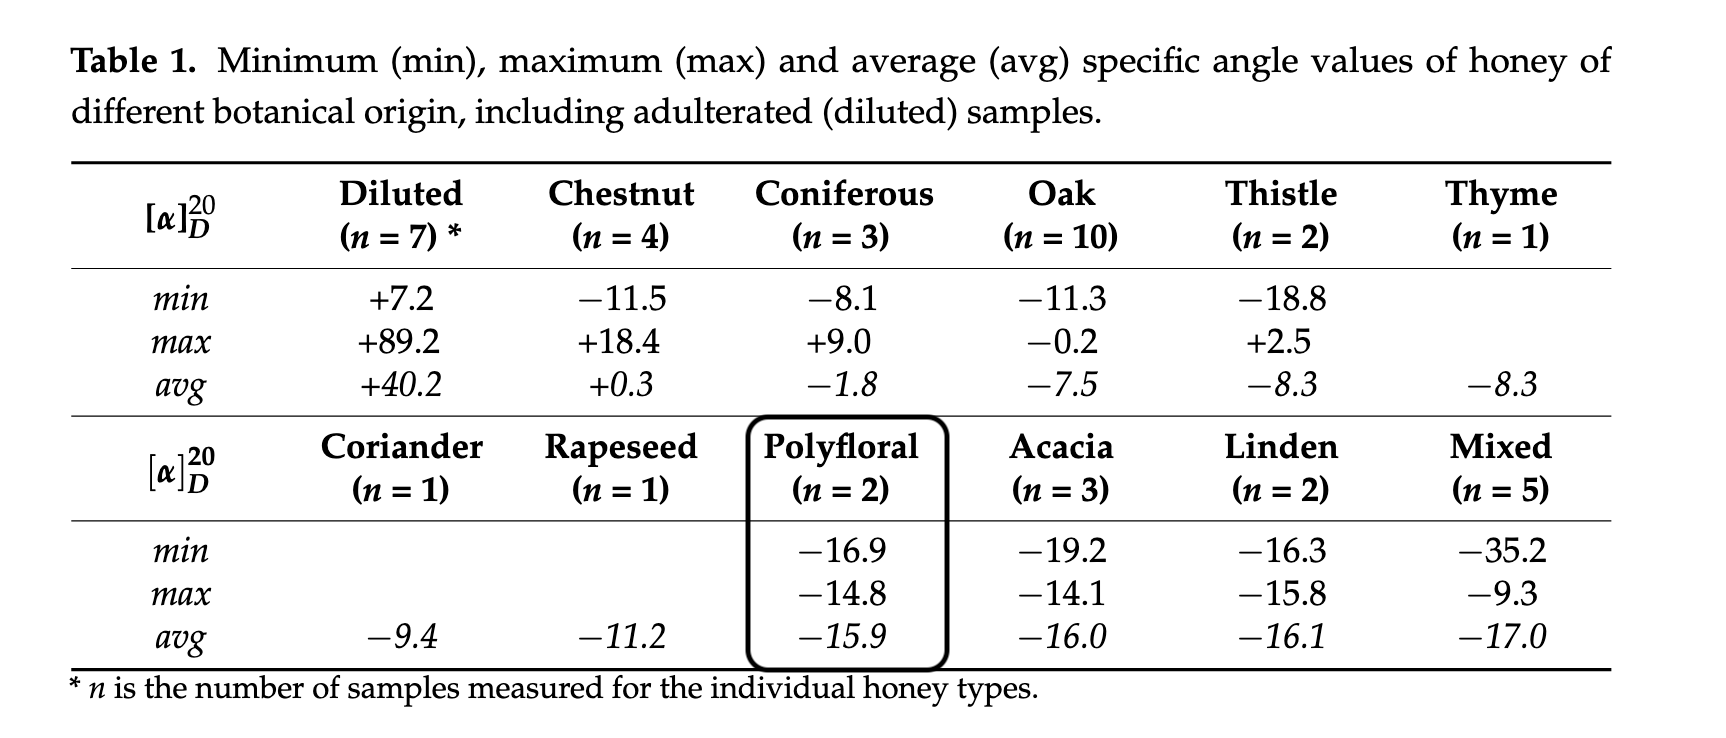
\includegraphics[width=1\textwidth]{slike/med.png}
\end{center}


Pri drugem medu (iz trgovine) pa smo dobili rezultat:

\[
    [\alpha]_{med_2} = \frac{\alpha}{c \cdot L} = \frac{3 ^\circ}{0.005 \cdot 11.5} = 52
\]
\[
    \sigma [\alpha]_{med_2} = 0,2 + 1 + 0,04 = 1,24 
\]

\begin{center}
\fbox{
    \begin{minipage}{0.8\textwidth}
        Rezultat za specifično rotacijo drugega medu:
        \[
            \abserr{[\alpha]}{med_2}{52}{65}{\frac{^\circ \cdot \mathrm{dm}}{\mathrm{g} \cdot \mathrm{mL}}}
        \]
        \[
            \relerr{[\alpha]}{med_2}{52}{1.24}{\frac{^\circ \cdot \mathrm{dm}}{\mathrm{g} \cdot \mathrm{mL}}}
        \]
    \end{minipage}
}
\end{center}


\begin{center}
    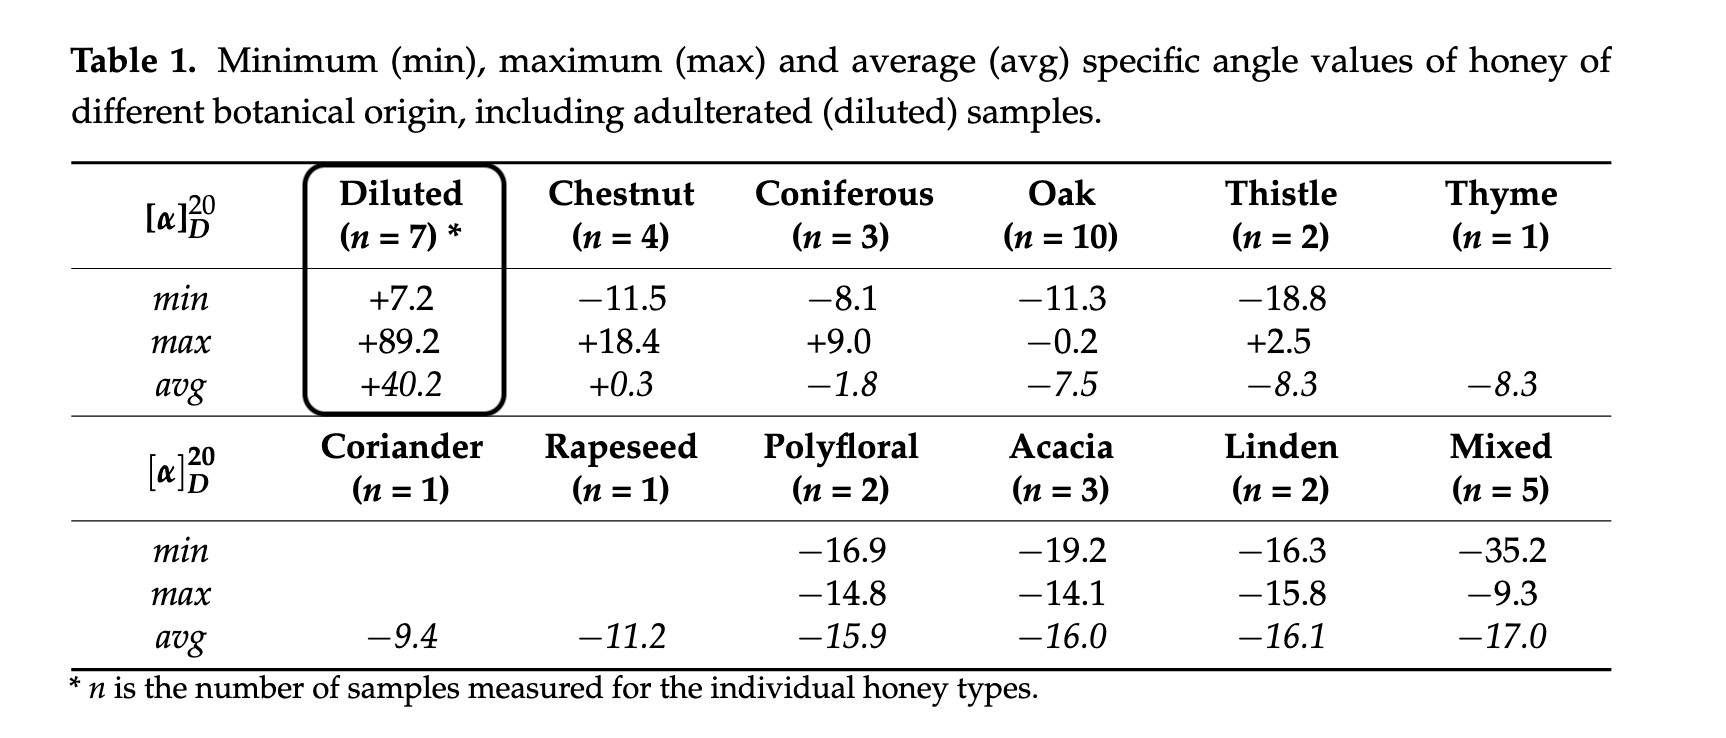
\includegraphics[width=1\textwidth]{slike/med2.png}
\end{center}

Zaradi gromozanske napake, ki je nastala, zaradi malega kota in velike absolutne napake kota, ne moremo v celoti trditi, da je med umeten. 
Vendar vseeno sumimo, da je temu tako, saj je med$_1$ kristaliziral med tem ko med$_2$ ni. 


\section*{Zaključek}

\bibliographystyle{plain}
\bibliography{predstavitev}

\end{document}